%!TEX root = ../../thesis.tex
\chapter{実験}
\label{chap:experiment}

本章では，構築したシステムが，データを収集していない環境でもシナリオに従って目的地まで移動できるかを，シミュレータ上で検証する．

\section{実験環境}
\label{sec:experiment_env}

実験環境として，千葉工業大学2号館3階の高層棟と低層棟を3次元再構成した2つのシミュレータ環境を用いる．
それぞれの環境を\figref{fig:sim_env}に示す．
高層棟を，データを収集した学習環境とし，低層棟を学習に用いない未学習環境とする．
両者は，床や壁の色，エレベーターの有無などの外観が異なる．
シナリオは高層棟7例，低層棟6例を用意する．各環境のシナリオと経路を\figref{fig:scenario}，\figref{fig:scenario_unseen}に，シナリオの文を\tabref{tab:scenarios}に示す．
シナリオには，直進のみのもの，左折と右折を含むもの，「左手に通路が見えるまで」のように方向を指定した条件を含むものがある．

\begin{table}[tb]
  \centering
  \caption{Scenarios used in the experiment}
  \label{tab:scenarios}
  \small
  \begin{tabular}{clp{0.72\linewidth}}
    \toprule
    No. & 環境 & シナリオ \\
    \midrule
    01 & 高層棟 & 3番目の三叉路まで直進．停止． \\
    02 & 高層棟 & 2番目の三叉路まで直進．左折．突き当りまで直進．停止． \\
    03 & 高層棟 & 突き当りまで直進．左折．左手に通路が見えるまで直進．左折．右手に通路が見えるまで直進．右折．左手に曲がり角が見えるまで直進．左折．突き当りまで直進．停止． \\
    04 & 高層棟 & 突き当りまで直進．左折．左手に通路が見えるまで直進．左折．右手に通路が見えるまで直進．右折．左手に曲がり角が見えるまで直進．左折．突き当りまで直進．右折．突き当りまで直進．停止． \\
    05 & 高層棟 & 右手に曲がり角が見えるまで直進．右折．突き当りまで直進．左折．突き当りまで直進．停止． \\
    06 & 高層棟 & 突き当りまで直進．右折．左手に通路が見えるまで直進．左折．三叉路まで直進．停止． \\
    07 & 高層棟 & 左を向く．突き当りまで直進．右折．右手に曲がり角が見えるまで直進．右折．突き当りまで直進．停止． \\
    08 & 低層棟 & 突き当りまで直進．停止． \\
    09 & 低層棟 & 左手に曲がり角が見えるまで直進．左折．突き当りまで直進．右折．突き当りまで直進．停止． \\
    10 & 低層棟 & 突き当りまで直進．左折．突き当りまで直進．停止． \\
    11 & 低層棟 & 突き当りまで直進．停止． \\
    12 & 低層棟 & 次の角まで直進．右折．突き当りまで直進．右折．突き当りまで直進．停止． \\
    13 & 低層棟 & 次の角まで直進．右折．突き当りまで直進．停止． \\
    \bottomrule
  \end{tabular}
\end{table}

% TODO: 要確認．シナリオの文は scenario_navigation/config/Scenarios/scenario{01..07,16,17,27,31,36,37}.txt から取った
%       （図のファイル名 Scenario_16.pdf などとの対応で，No.08〜13 に振り直している）．

シミュレータにはGazeboを用い，ロボットの前方に取り付けた1台のカメラの画像を各モジュールへ入力する．

% TODO: ロボットのモデル，カメラの解像度と画角，学習と推論に用いた計算機を書く．

\begin{figure}[tb]
  \centering
  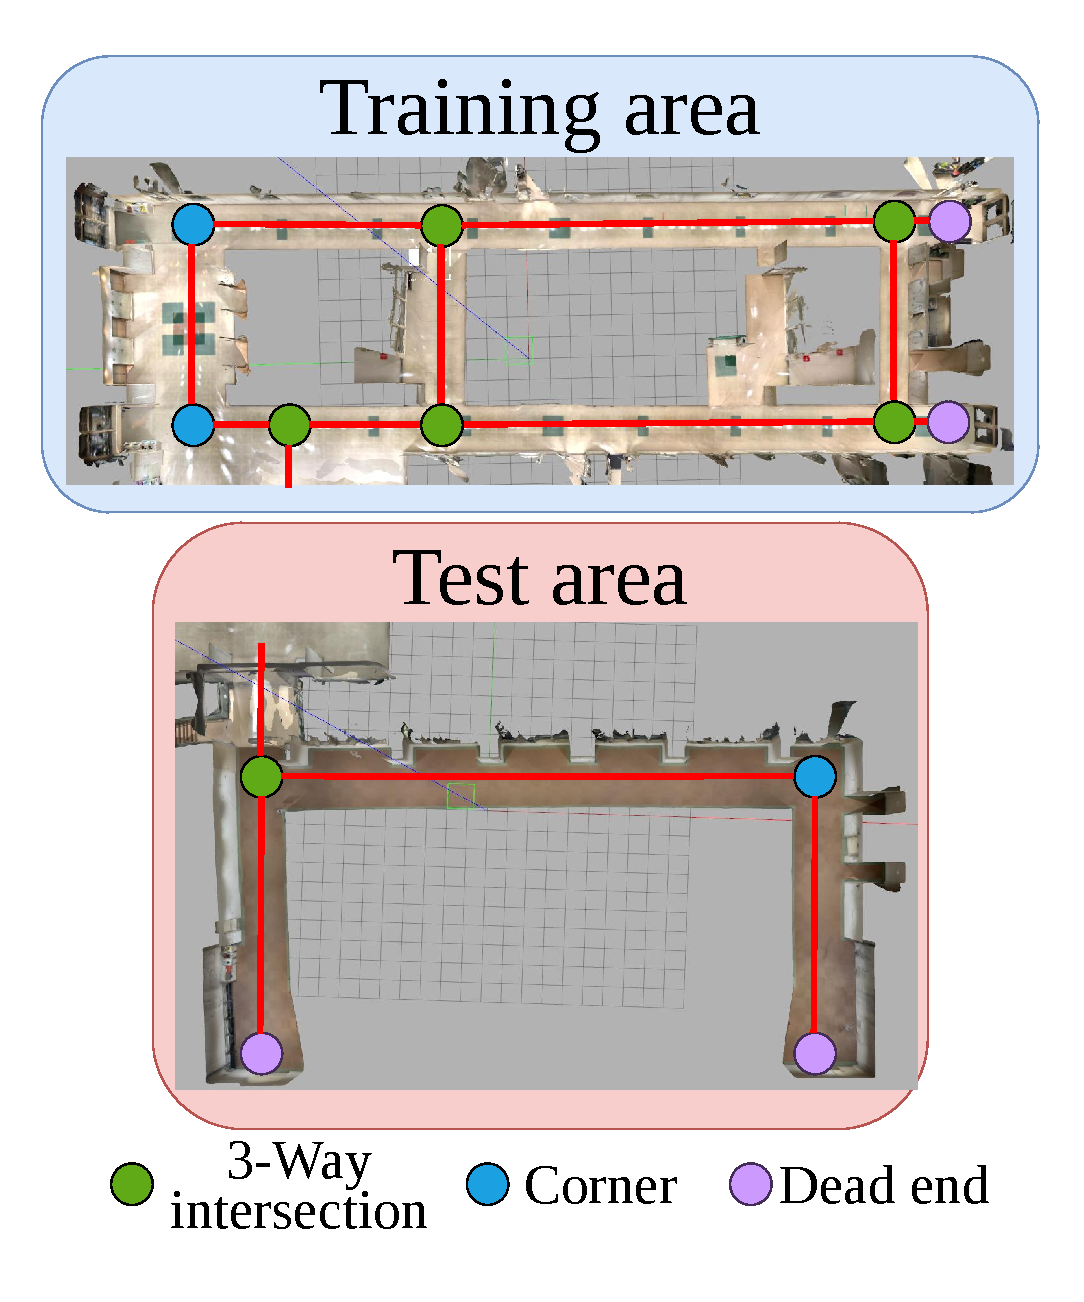
\includegraphics[width=0.86\linewidth]{images/enviroment.pdf}
  \caption{Simulator environments}
  \label{fig:sim_env}
\end{figure}

\section{データセット}
\label{sec:dataset}

データセットは，学習環境である高層棟でのみ作成する．
ROS navigationパッケージにより経由点列に沿ってロボットを走行させ，走行中のカメラ画像，自己位置および目標方向を$0.25$\,s間隔で記録する．
経由点にはあらかじめ通路形状と目標方向を設定し，記録時に各カメラ画像へ対応するラベルを自動的に付与する．
これにより，手動でラベルを付与することなく，データセットを構築できる．
高層棟を約$\SI{395}{m}$走行し，計$6069$サンプルを得た．
内訳を\tabref{tab:dataset}に示す．

通路分類モジュールの入力は$224\times224$に，経路追従モジュールの入力は$96\times96$にリサイズする．
経路追従の教師は，記録した自己位置から，各時刻のロボット座標系における$8$点のwaypoint列として算出する．

通路分類のラベルは，経由点に設定した通路形状を，次の経由点に到達するまでの画像に付与する．
ただし，旋回中の画像は通路形状が定まらないため，ロボットの角速度から旋回中と判定した区間を通路形状の学習から除く．
目標方向のラベルは，直進が全体の約7割を占め，左折と右折はそれぞれ約1.5割である（\tabref{tab:dataset}）．
通路形状も一本道が約半数を占め，行き止まりは48サンプルと少ない．

% TODO: 要確認．ラベル付けの規則（旋回区間の扱い）は corridor_classifier/config/dataset.yaml の turn_detection から推測したもの．

\begin{table}[tb]
  \centering
  \caption{Training dataset collected in the high-rise wing}
  \label{tab:dataset}
  \begin{tabular}{lr@{\qquad}lr}
    \toprule
    Passage class & Samples & Target direction & Samples \\
    \midrule
    straight\_road & 3140 & straight & 4269 \\
    3\_way\_left   &  738 & left     &  908 \\
    3\_way\_right  &  727 & right    &  892 \\
    3\_way\_center &  620 &          &      \\
    corner\_right  &  399 &          &      \\
    corner\_left   &  397 &          &      \\
    dead\_end      &   48 &          &      \\
    \midrule
    Total & 6069 & Total & 6069 \\
    \bottomrule
  \end{tabular}
\end{table}

\section{実験方法}
\label{sec:experiment_method}

実験は以下の手順で行う．
通路分類モデルと経路追従モデルは，高層棟のデータで1度だけ学習し，両方の環境で同じモデルを用いる．
\begin{enumerate}[label=\arabic*)]
  \item ROS navigationパッケージでロボットを走行させ，データを収集する．
  \item 収集したデータセットを用いて，通路分類モデルと経路追従モデルをファインチューニングする．
  \item シナリオの開始地点にロボットを配置する．
  \item シナリオを入力し，自律移動を開始する．
  \item 目的地へ到達するかを確認する．
\end{enumerate}

% TODO: 各シナリオの試行回数，成功の判定基準，記録する項目を書く．

\begin{figure}[p]
  \centering
  \begin{subfigure}[b]{0.32\linewidth}
    \centering
    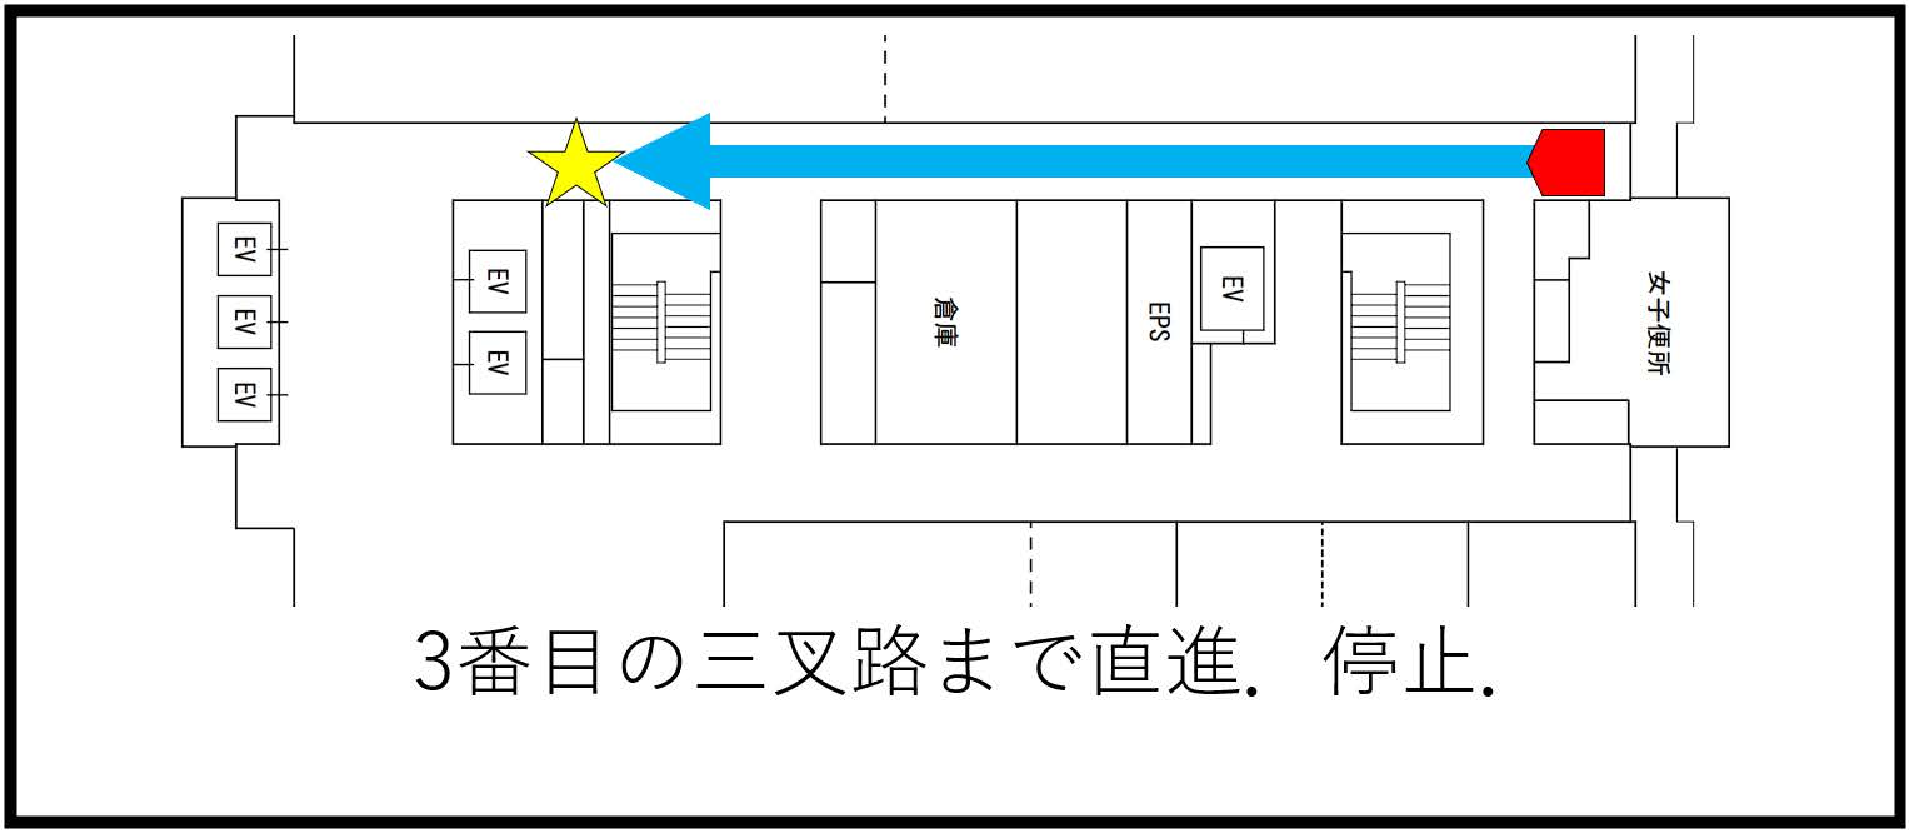
\includegraphics[width=\linewidth]{images/Scenario_01.pdf}
    \caption{Scenario 01}
  \end{subfigure}\hfill
  \begin{subfigure}[b]{0.32\linewidth}
    \centering
    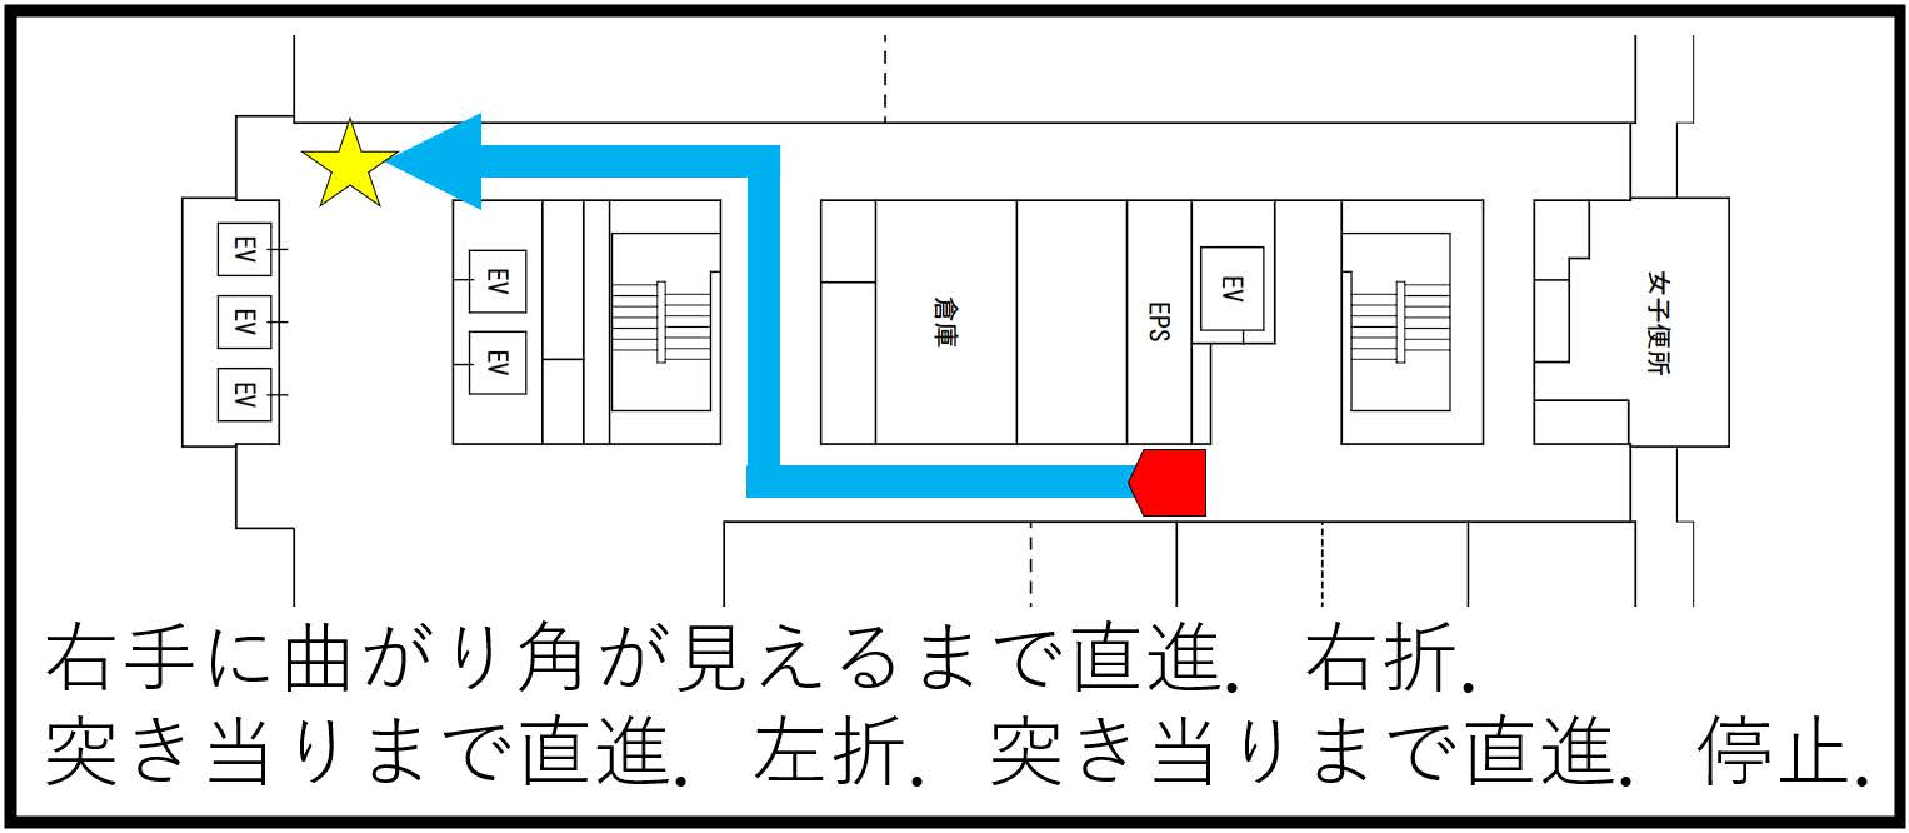
\includegraphics[width=\linewidth]{images/Scenario_02.pdf}
    \caption{Scenario 02}
  \end{subfigure}\hfill
  \begin{subfigure}[b]{0.32\linewidth}
    \centering
    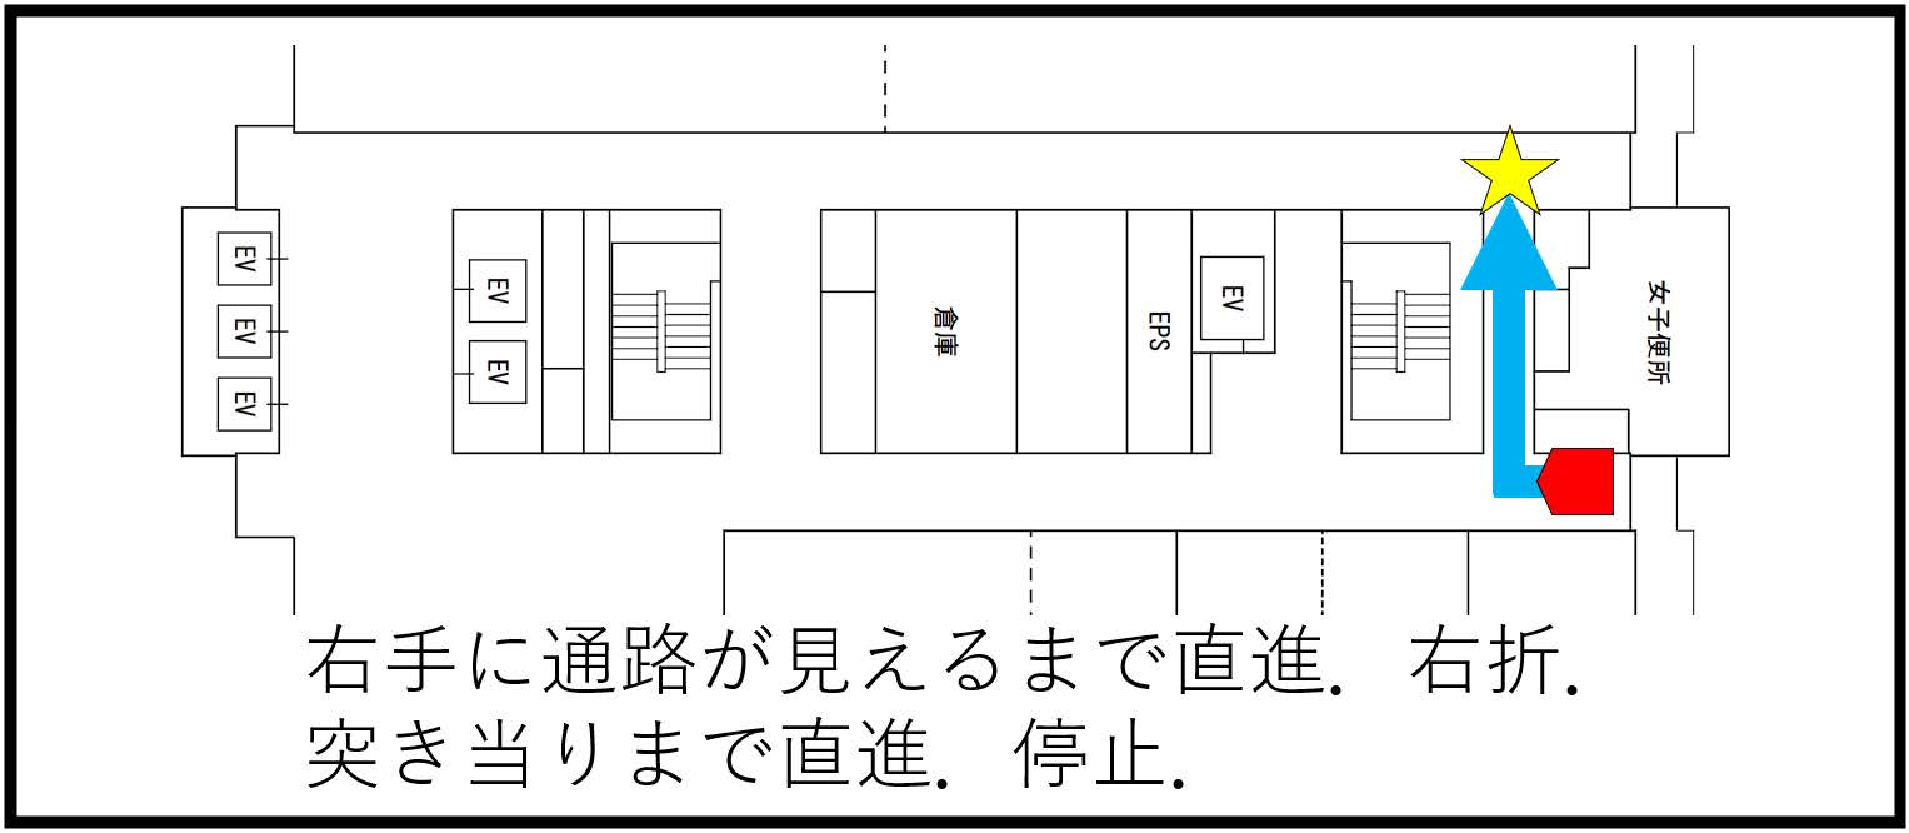
\includegraphics[width=\linewidth]{images/Scenario_03.pdf}
    \caption{Scenario 03}
  \end{subfigure}

  \vspace{0.5\baselineskip}

  \begin{subfigure}[b]{0.32\linewidth}
    \centering
    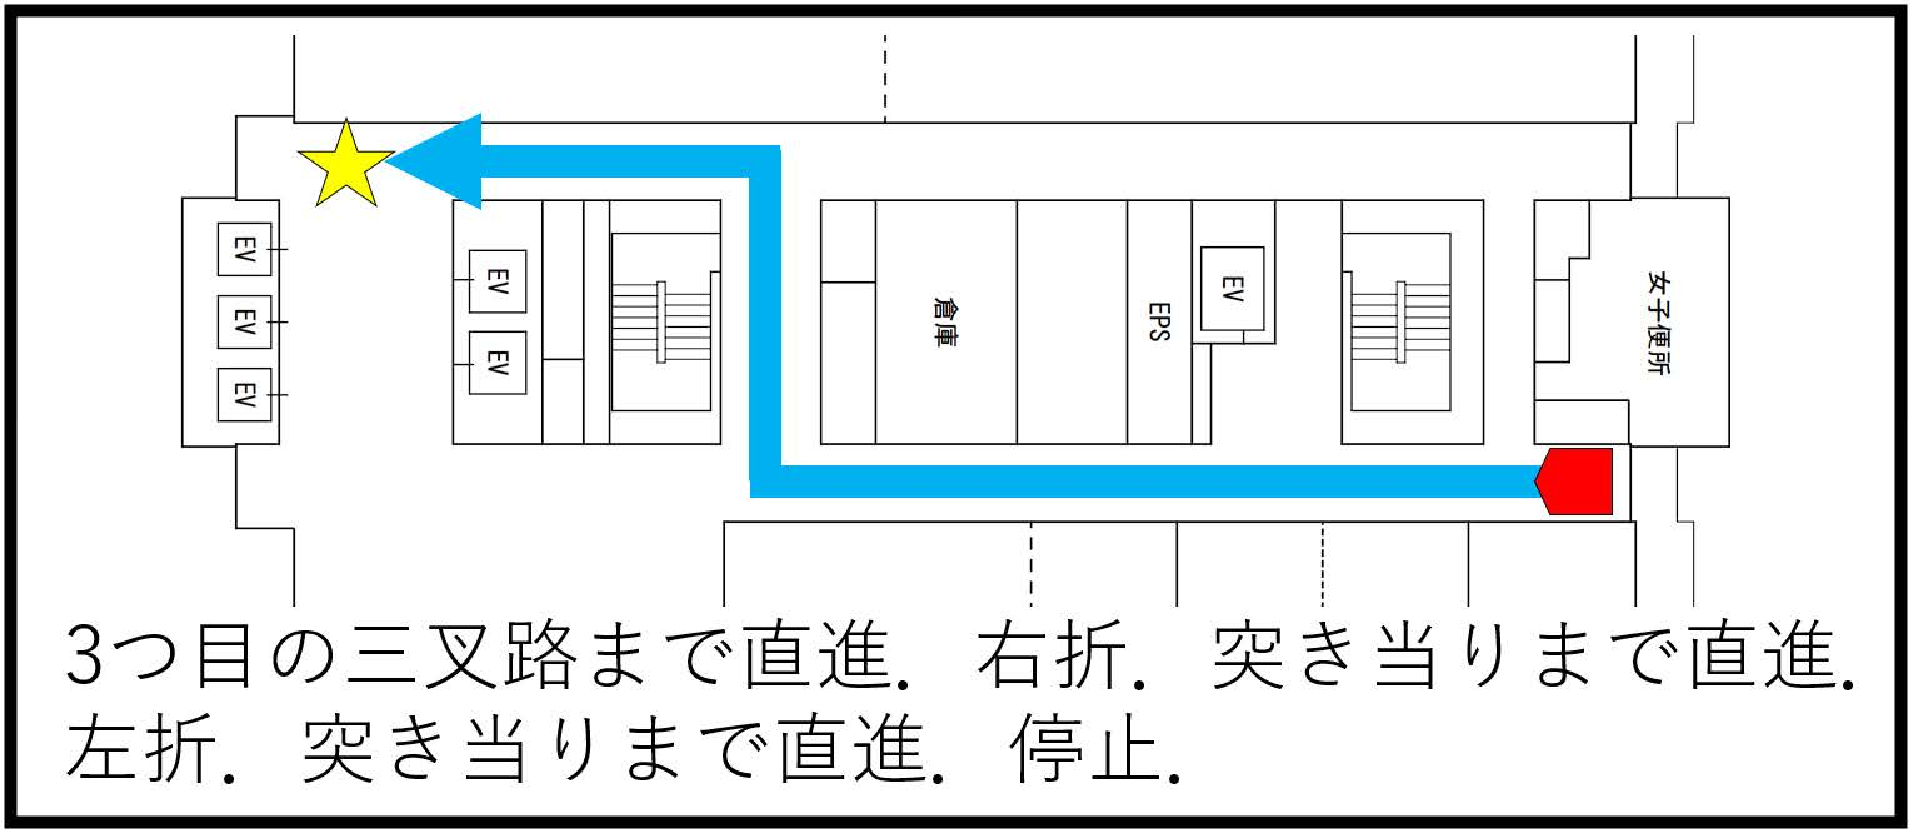
\includegraphics[width=\linewidth]{images/Scenario_04.pdf}
    \caption{Scenario 04}
  \end{subfigure}\hfill
  \begin{subfigure}[b]{0.32\linewidth}
    \centering
    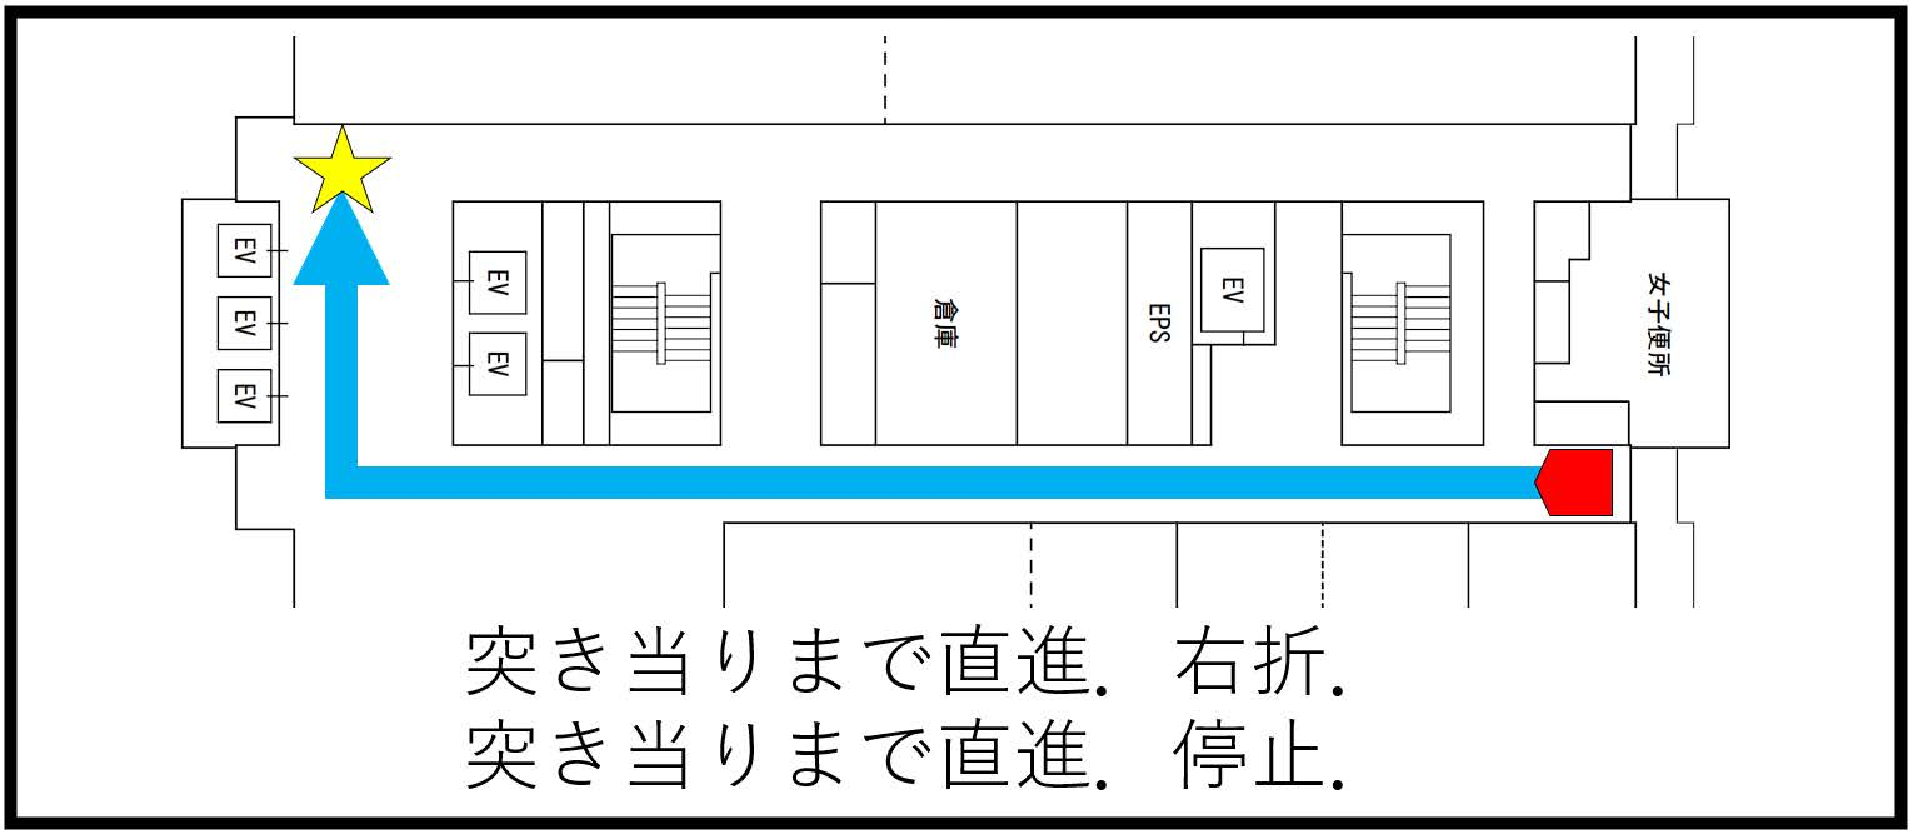
\includegraphics[width=\linewidth]{images/Scenario_05.pdf}
    \caption{Scenario 05}
  \end{subfigure}\hfill
  \begin{subfigure}[b]{0.32\linewidth}
    \centering
    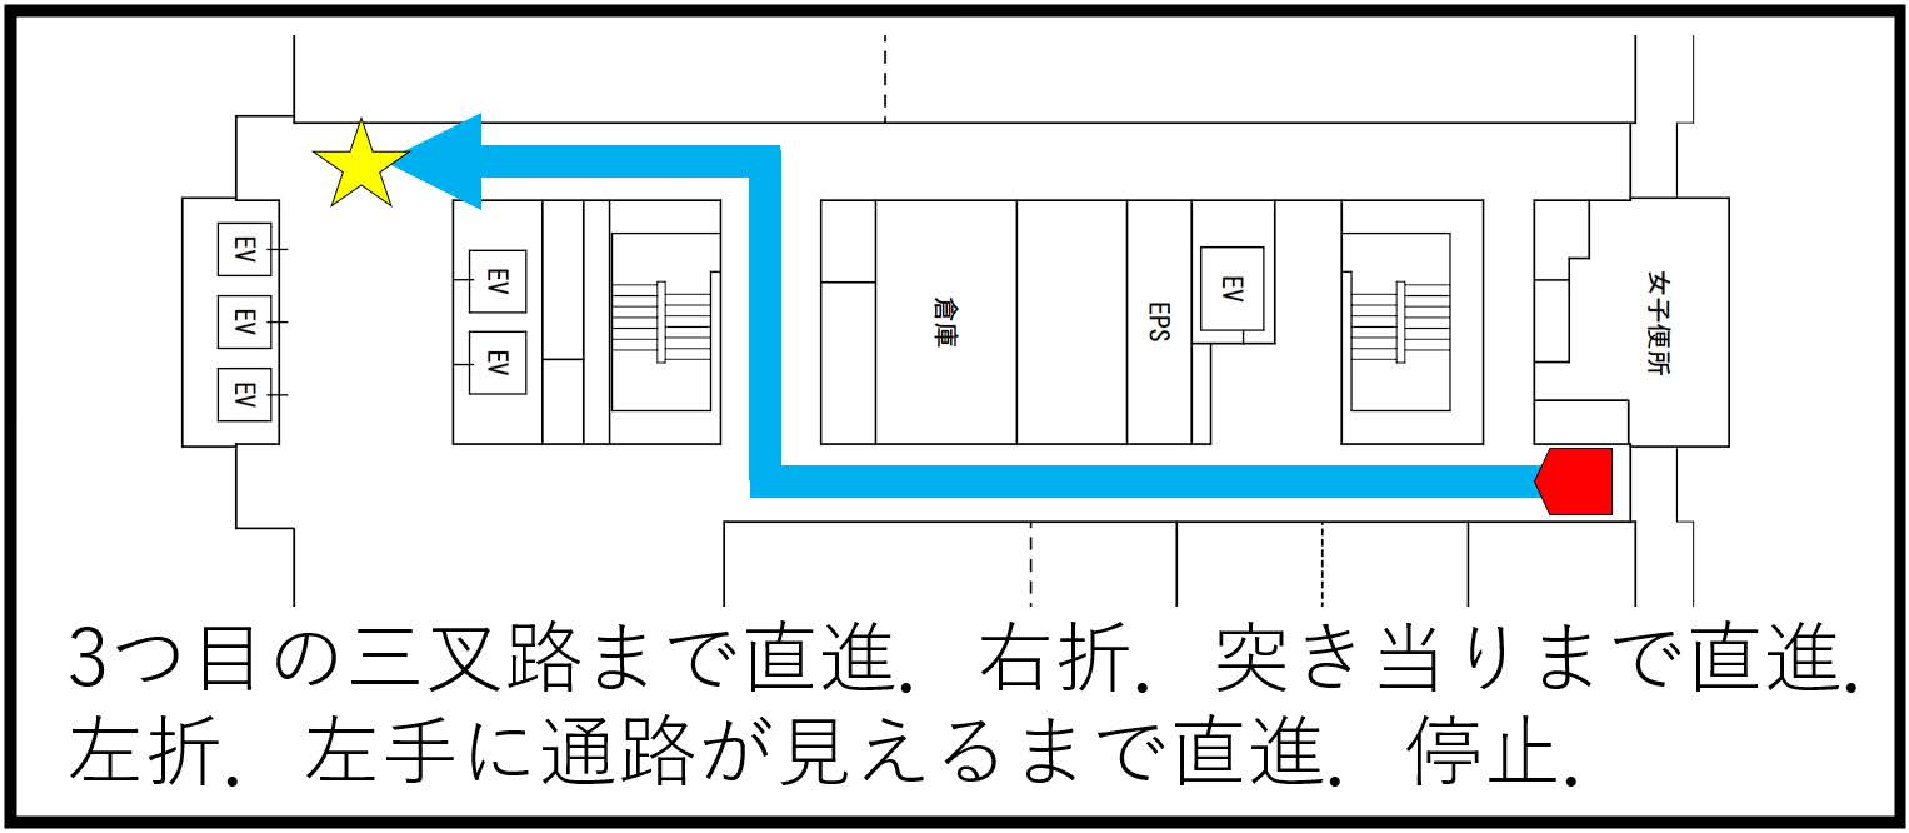
\includegraphics[width=\linewidth]{images/Scenario_06.pdf}
    \caption{Scenario 06}
  \end{subfigure}

  \vspace{0.5\baselineskip}

  \begin{subfigure}[b]{0.32\linewidth}
    \centering
    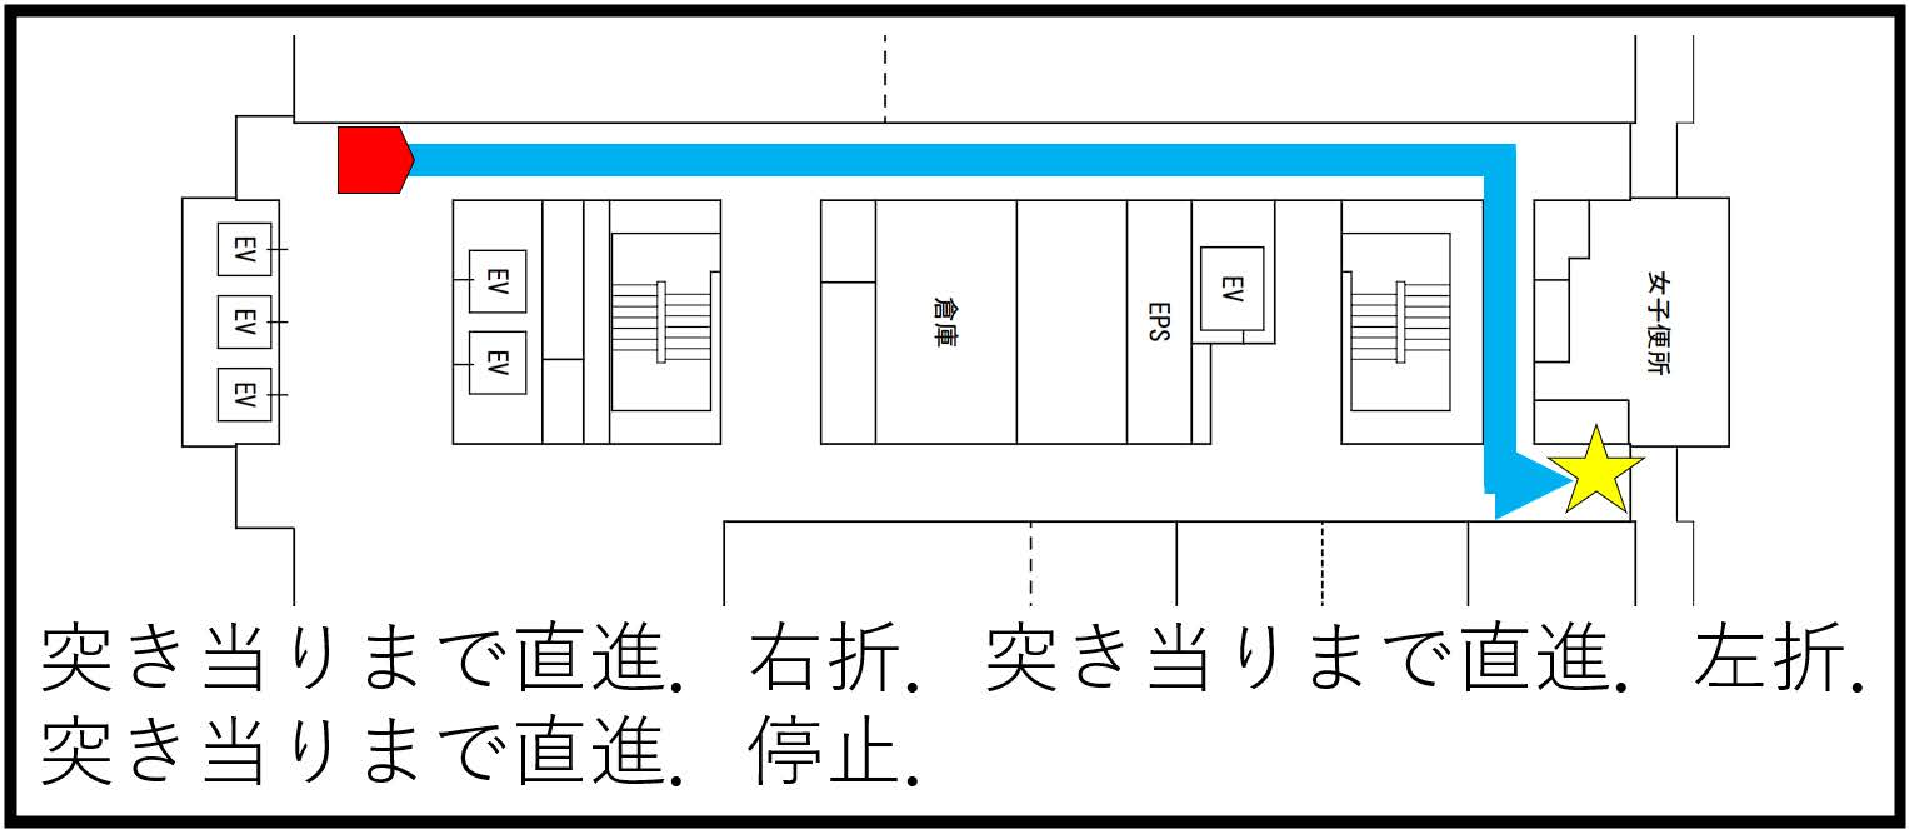
\includegraphics[width=\linewidth]{images/Scenario_07.pdf}
    \caption{Scenario 07}
  \end{subfigure}
  \caption{Scenarios used in the training environment}
  \label{fig:scenario}
\end{figure}

\begin{figure}[p]
  \centering
  \begin{subfigure}[b]{0.32\linewidth}
    \centering
    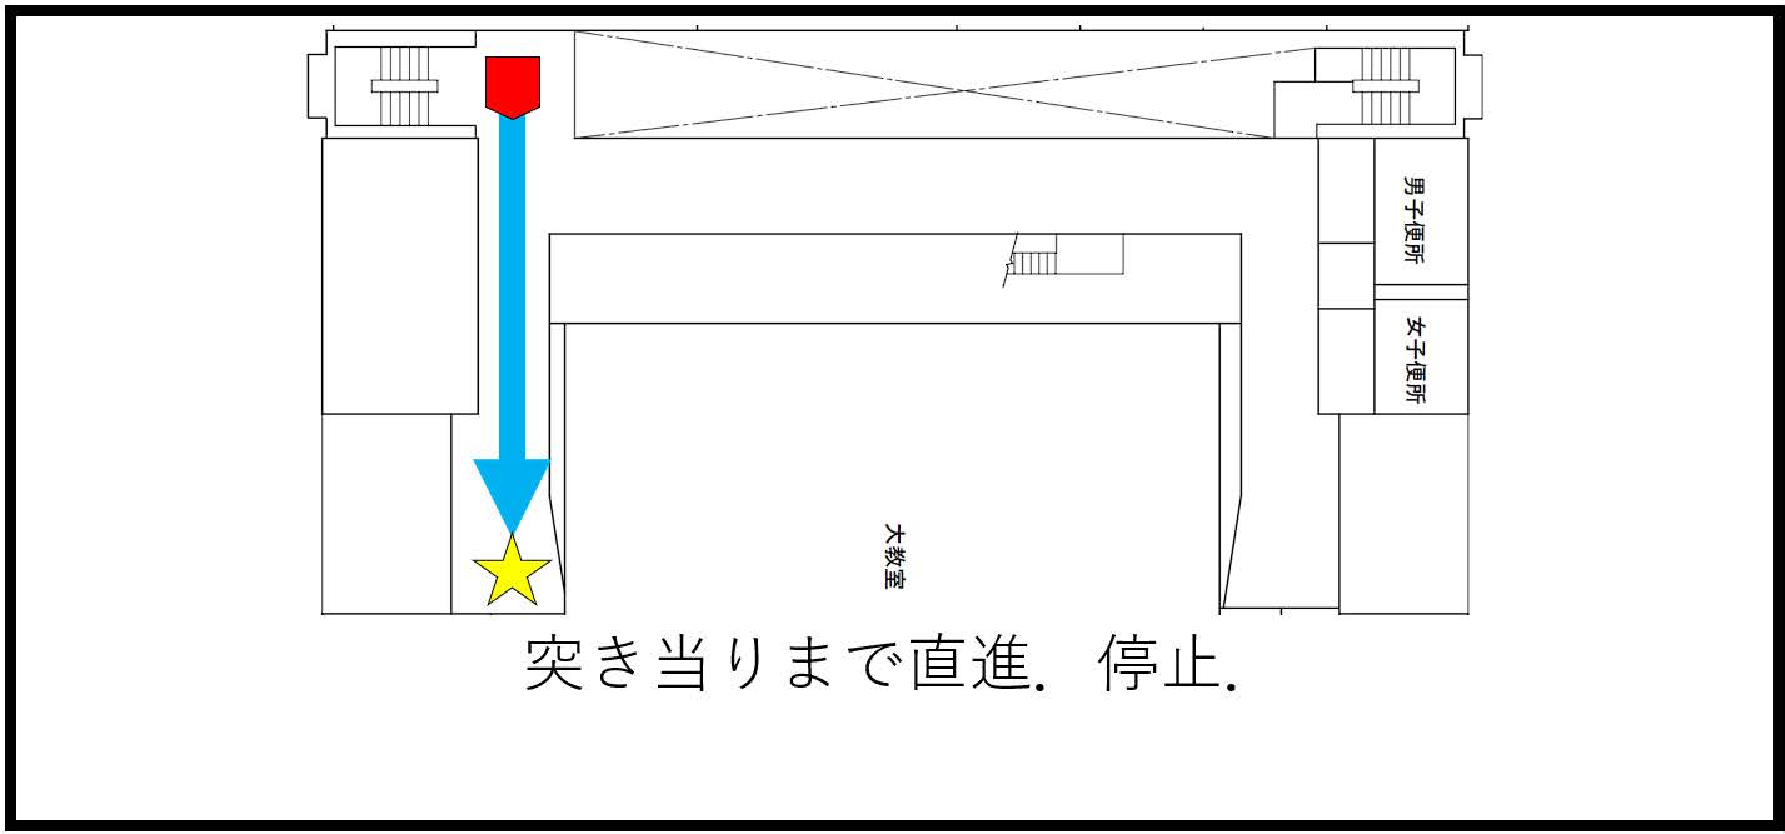
\includegraphics[width=\linewidth]{images/Scenario_16.pdf}
    \caption{Scenario 08}
  \end{subfigure}\hfill
  \begin{subfigure}[b]{0.32\linewidth}
    \centering
    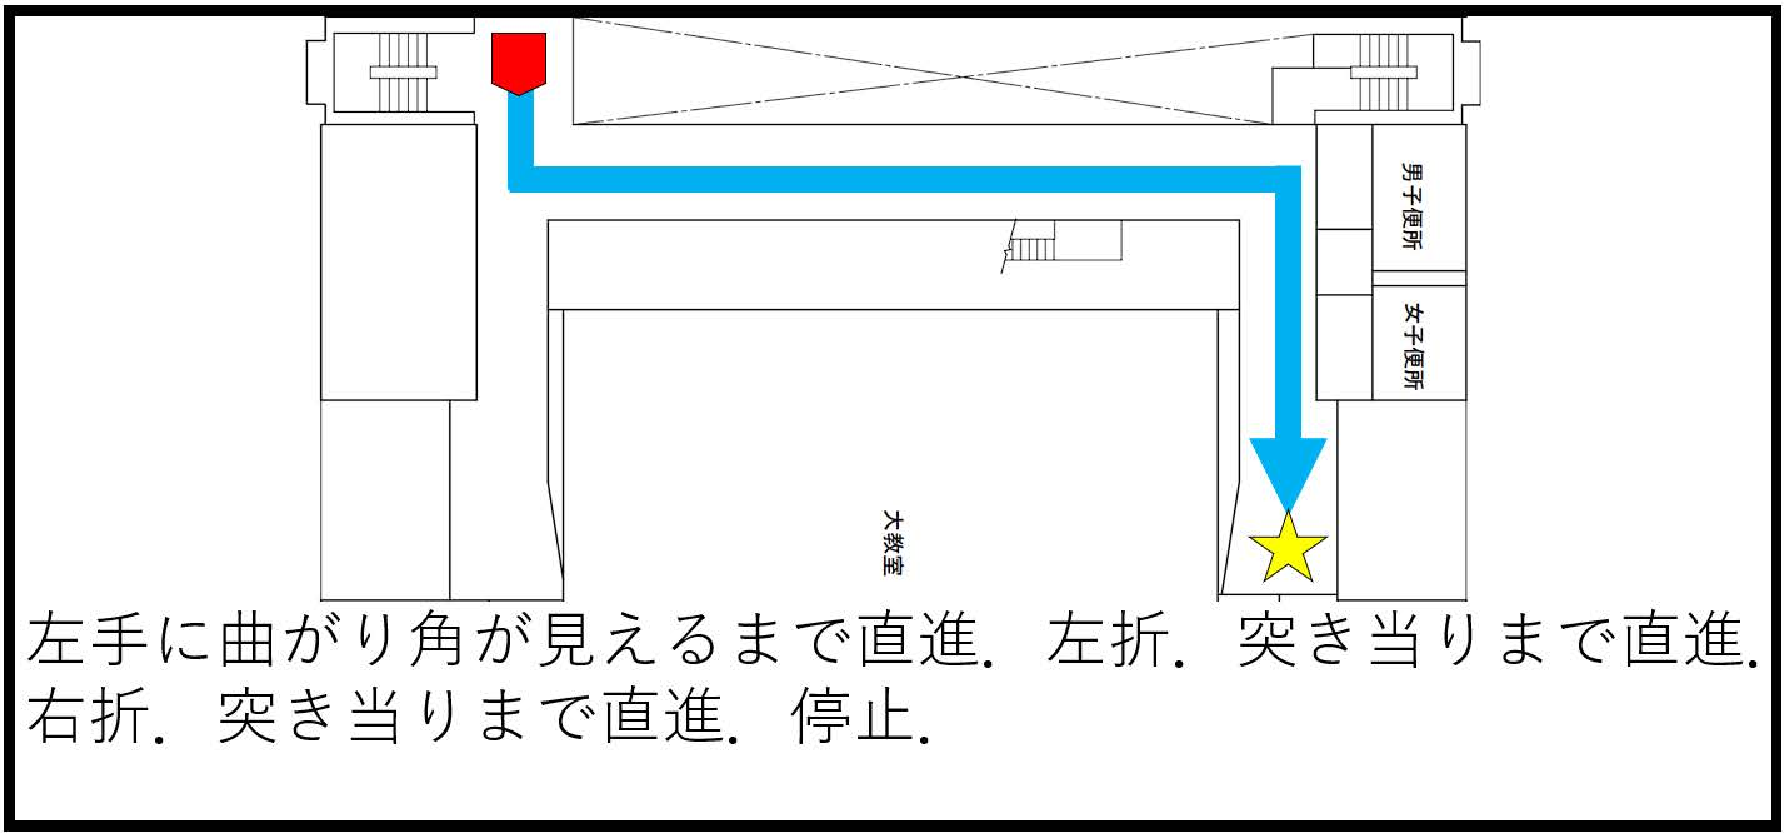
\includegraphics[width=\linewidth]{images/Scenario_17.pdf}
    \caption{Scenario 09}
  \end{subfigure}\hfill
  \begin{subfigure}[b]{0.32\linewidth}
    \centering
    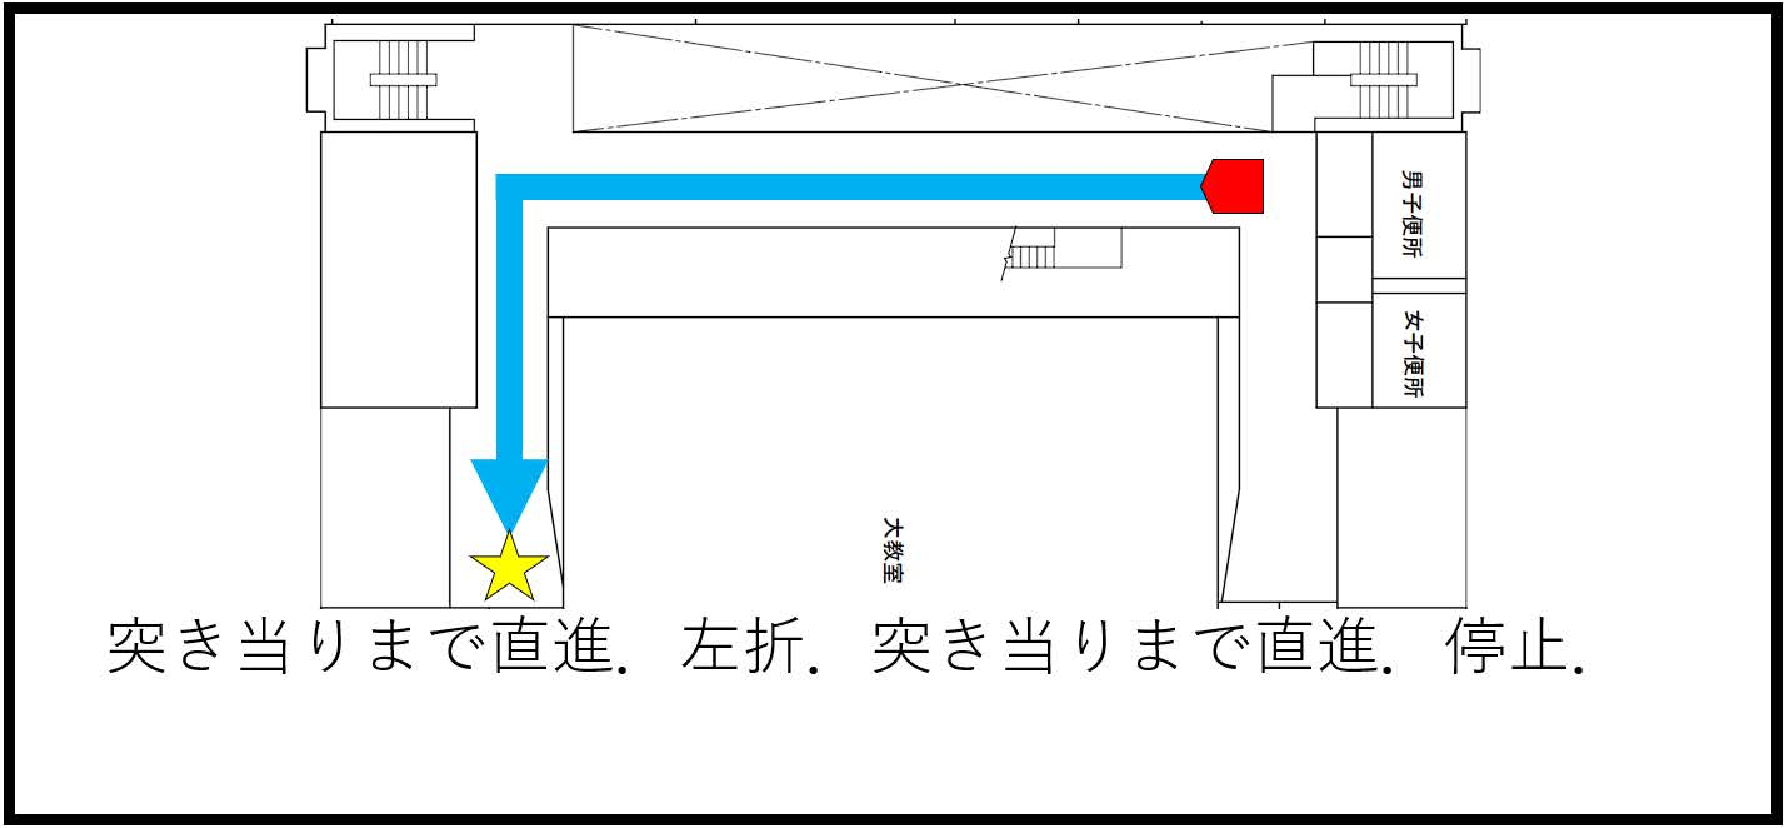
\includegraphics[width=\linewidth]{images/Scenario_27.pdf}
    \caption{Scenario 10}
  \end{subfigure}

  \vspace{0.5\baselineskip}

  \begin{subfigure}[b]{0.32\linewidth}
    \centering
    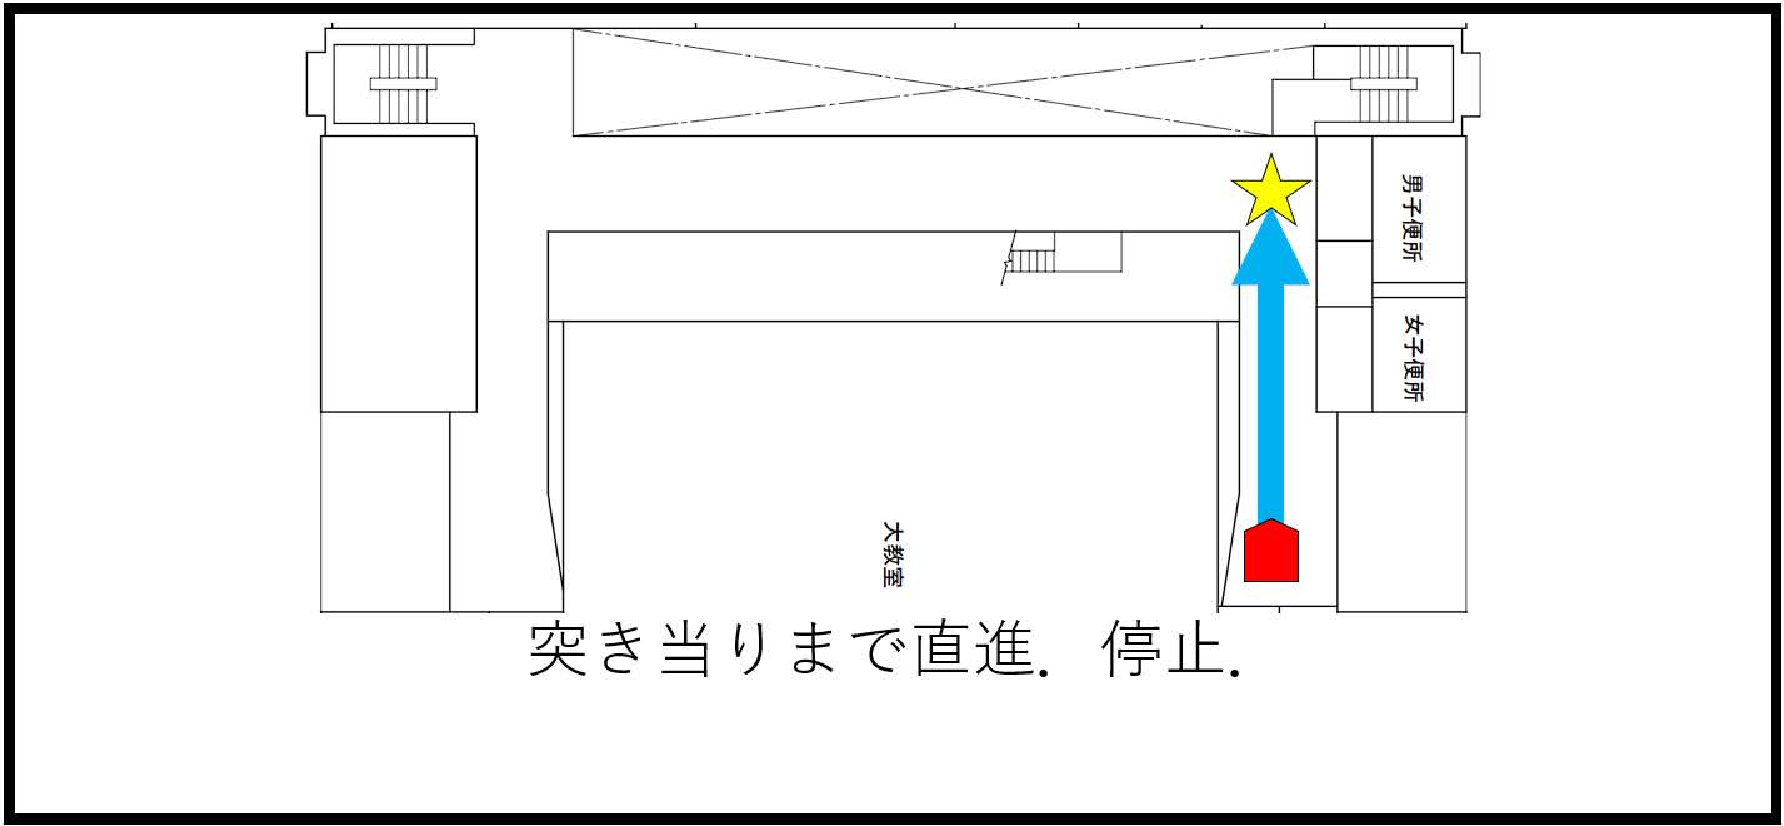
\includegraphics[width=\linewidth]{images/Scenario_31.pdf}
    \caption{Scenario 11}
  \end{subfigure}\hfill
  \begin{subfigure}[b]{0.32\linewidth}
    \centering
    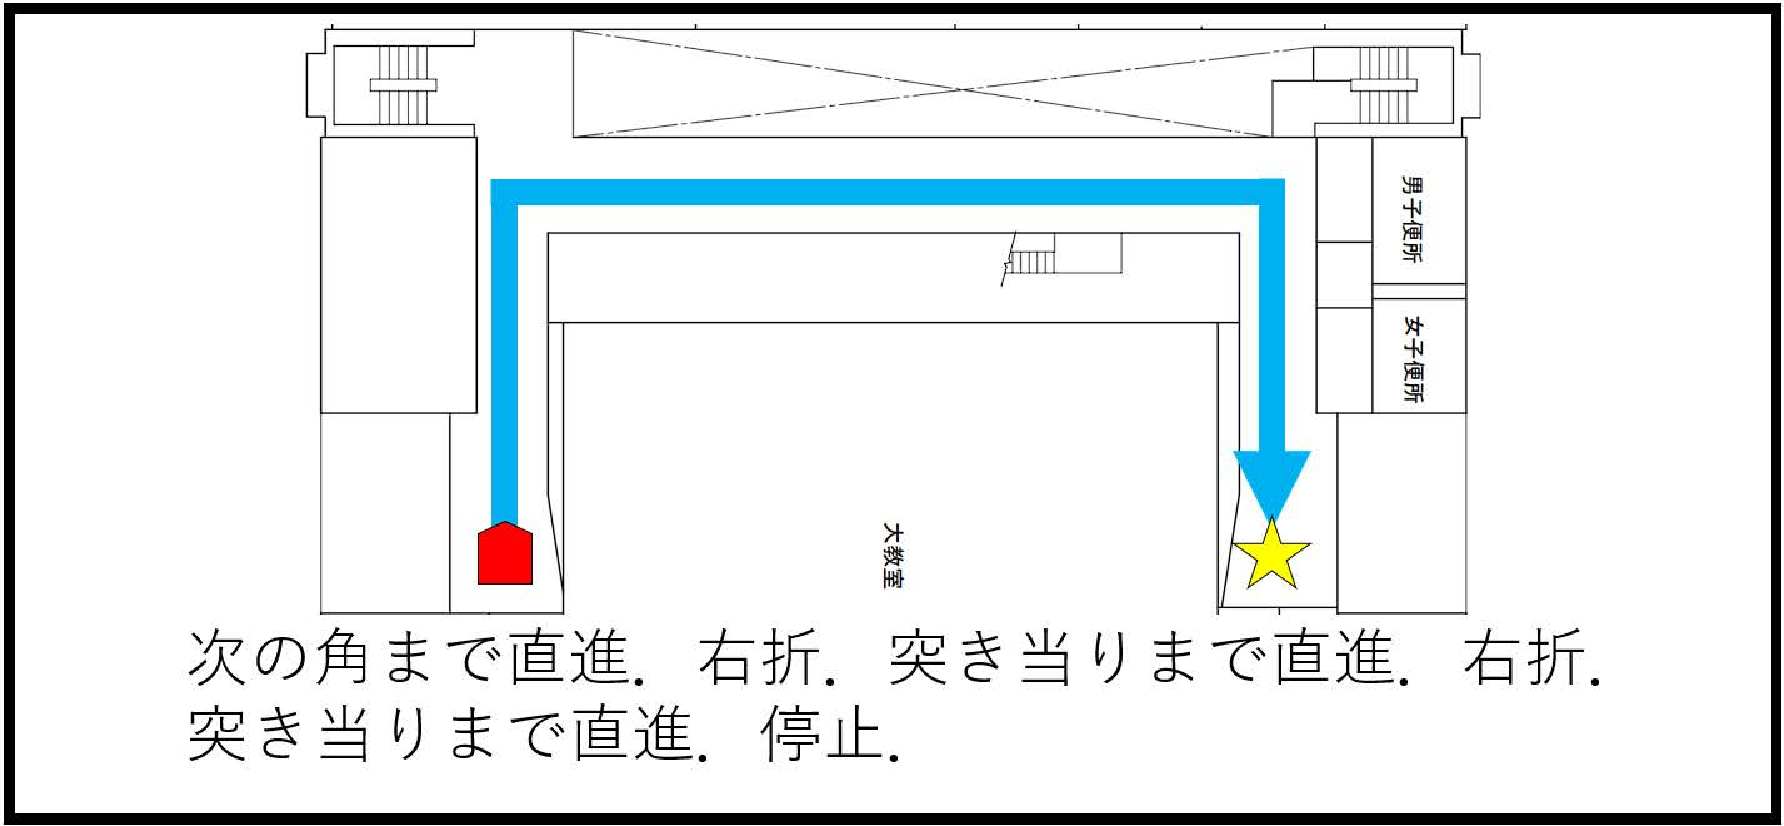
\includegraphics[width=\linewidth]{images/Scenario_36.pdf}
    \caption{Scenario 12}
  \end{subfigure}\hfill
  \begin{subfigure}[b]{0.32\linewidth}
    \centering
    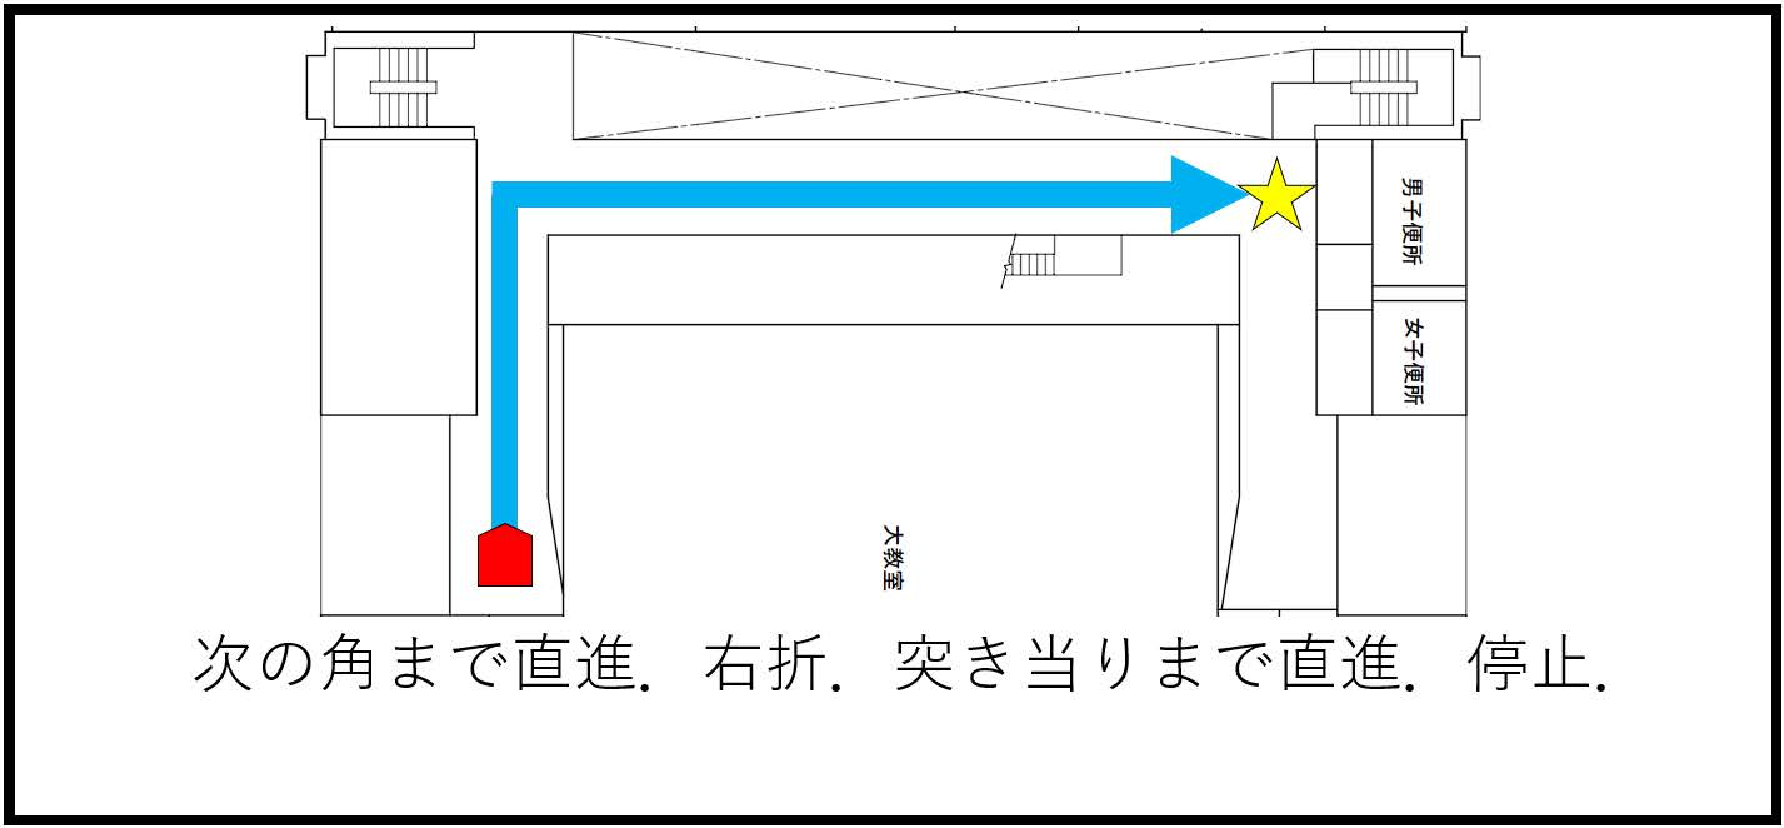
\includegraphics[width=\linewidth]{images/Scenario_37.pdf}
    \caption{Scenario 13}
  \end{subfigure}
  \caption{Scenarios used in the unseen environment}
  \label{fig:scenario_unseen}
\end{figure}

\section{実験結果}
\label{sec:experiment_result}

未学習環境である低層棟でのシナリオ09の走行の様子を\figref{fig:experiment}に示す．
実験の結果，13例すべてのシナリオにおいて，ロボットは目的地まで到達した．
学習環境である高層棟の7例に加え，学習に用いていない低層棟の6例でも到達した．

シナリオ09は，左手の曲がり角まで直進して左折し，突き当りで右折して，次の突き当りで停止する経路である．
このシナリオでは，「左手に曲がり角が見えるまで」と「突き当りまで」の2種類の条件を，未学習環境の画像から判定する必要がある．
% TODO: シナリオ09の走行で，各条件がどこで成立したかを走行ログから書く．

% TODO: シナリオごとの結果（到達の成否，走行時間，衝突の有無など）を表にする．

% TODO: si-paper ではこの図は差し替え予定とされていた（実環境の写真だが，実験はシミュレータ）．
\begin{figure}[tb]
  \centering
  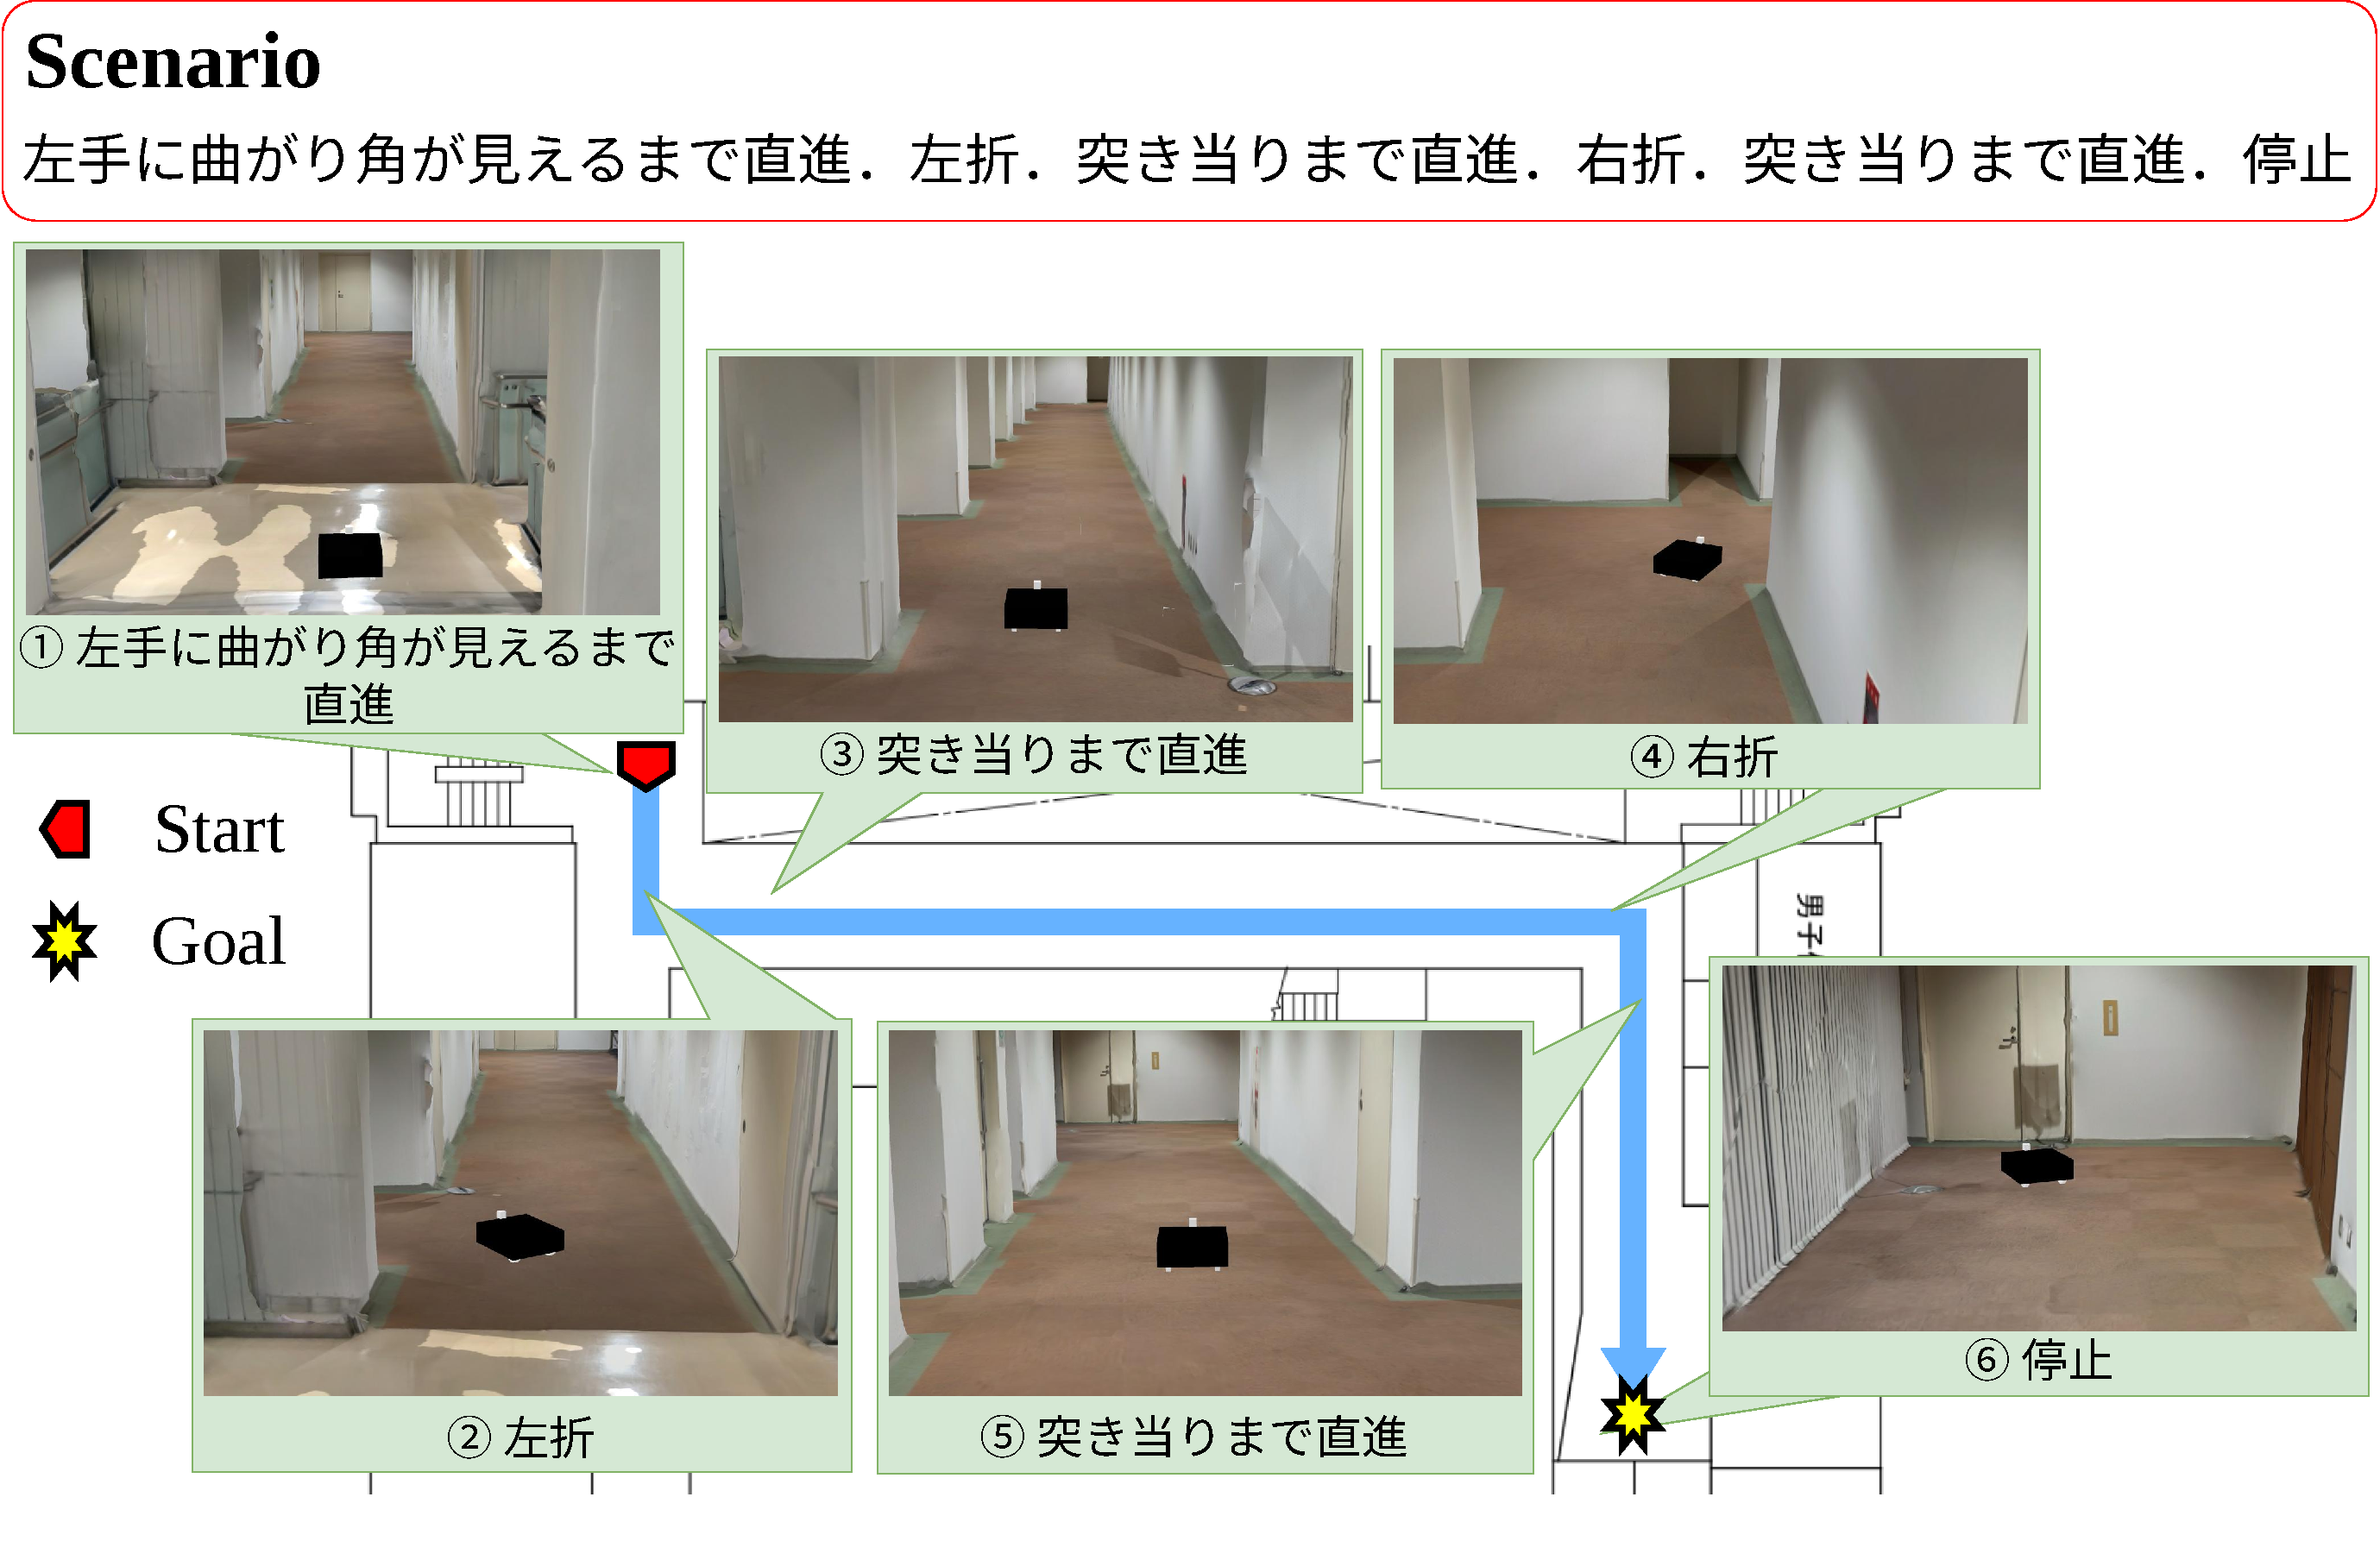
\includegraphics[width=\linewidth]{images/experiment.pdf}
  \caption{Navigation with Scenario 09 in the unseen environment}
  \label{fig:experiment}
\end{figure}

\section{考察}
\label{sec:discussion}

低層棟ではデータ収集やファインチューニングを一切行っていないことから，シミュレータ上の限られた例ではあるが，走行対象の環境でデータ収集や再学習を行わずに，シナリオに従って目的地まで移動できることを確認した．

本実験では，高層棟と低層棟で床や壁の色，エレベーターの有無などの外観が異なる．
それにもかかわらず未学習環境で目的地に到達できた要因として，次の2点が考えられる．
1点目は，\DINOvTwo と\NoMaD の視覚エンコーダを凍結し，事前学習で獲得された表現を保ったことである．
これにより，高層棟の外観に特化した特徴を学習することを避けられたと考えられる．
2点目は，\UniDepth の推定深度から求めた占有格子を通路分類に併用したことである．
占有格子は壁面の位置のみを表し，色や模様の情報を含まないため，外観が異なっても通路の形状を捉えられると考えられる．

一方で，本実験はシミュレータ上の13例に限られる．
また，上記の要因はそれぞれの構成要素を除いた比較を行っていないため，効果を定量的に示したものではない．
実環境では照明の変化や人の往来など，シミュレータにない要因があるため，実環境での評価が必要である．

% TODO: 基盤モデルを凍結した効果，BEVを併用した効果，CAREの効果を比較実験で示すか検討する．
%       corridor_classifier/config/experiments/ に比較の記録（BEV_REPRESENTATION_DECISION.md など）があるので，使えるか確認する．
